% Chapter 25: Mendelian Randomization
% A First Course in Causal Inference - Peng Ding
% Rewrite V1 - Stein-style narrative

\chapter{孟德尔随机化}\label{ch:25}

\section{引言：遗传学与因果推断的交汇}\label{sec:25-intro}

在第 \ref{ch:21} 章和第 \ref{ch:23} 章中，我们看到了工具变量（IV）方法如何帮助解决观测性研究中的未测量混杂问题。然而，传统 IV 方法面临一个根本困难：找到一个有效的工具变量谈何容易。研究者需要确信这个变量满足三个关键条件——与治疗变量相关、不与未测量混杂相关、以及仅通过治疗变量影响结果。

20 世纪 80 年代，一位名叫 Katan 的研究者 \citep{Katan1986} 提出了一个颇具洞察力的观点：也许遗传变异能够充当天然的工具变量。他的论证基于孟德尔的第二定律——独立分配定律（law of random assortment），该定律表明一种性状的遗传独立于其他性状的遗传。这意味着，如果我们能找到与某个暴露因素（如胆固醇水平）相关的基因变异，同时这些变异与混杂暴露因素与结果之间关系的未测量混杂因子相互独立，那么这些基因变异就可能成为一个有效的工具变量。

这一思想在流行病学研究中引发了革命性的变革。2003 年，Davey Smith 和 Ebrahim \citep{DaveySmith2003} 将这种方法正式命名为\textbf{孟德尔随机化（Mendelian Randomization, MR）}。如今，MR 已成为流行病学中估计暴露因素对结果因果效应的核心方法 \citep{VanderWeele2014}。

\textbf{本章的核心问题}：如何利用遗传变异作为工具变量来估计因果效应？这种方法的假设是什么？又有哪些局限性？

\section{背景与动机}\label{sec:25-background}

\subsection{从胆固醇到癌症：一个经典难题}\label{sec:25-cholesterol-example}

在深入技术细节之前，让我们先理解 MR 最初被提出时的动机。20 世纪 80 年代的观测性研究暗示，低血清胆固醇水平可能与癌症风险相关。然而，这样的观察性研究面临两个根本性问题：

\begin{enumerate}
  \item \textbf{未测量的混杂}：胆固醇水平和癌症之间可能存在共同的未测量混杂因素，例如饮食模式或社会经济地位。
  \item \textbf{反向因果}：更棘手的是，癌症的早期阶段可能反过来导致低血清胆固醇水平，即因果方向可能与假设的相反。
\end{enumerate}

Katan \citep{Katan1986} 指出，Apolipoprotein E 基因与血清胆固醇水平相关，但（理论上）不直接影响癌症状态。因此，如果我们能比较携带不同基因型的人群在癌症风险上的差异，就能区分因果效应和混杂/反向因果。这一论证与我们在第 \ref{ch:21} 章讨论的 IV 框架完美契合。

\subsection{MR 的因果图}\label{sec:25-causal-graph}

图 \ref{fig:25-mr-causal-graph} 展示了一个典型 MR 研究的因果结构。

\begin{figure}[htbp]
\centering
% 因果图示意（用 tikz 绘制）
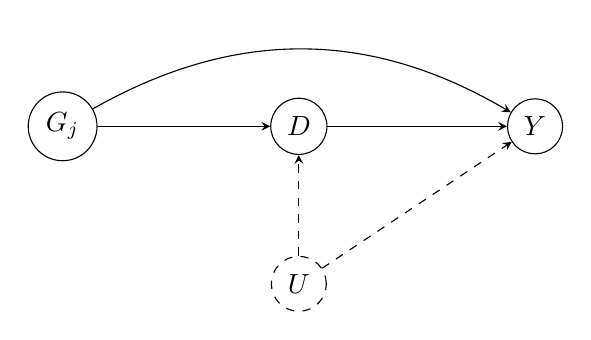
\begin{tikzpicture}[>=stealth, node distance=1.5cm]
  % 节点定义
  \node[circle, draw] (G) at (-3, 0) {$G_j$};
  \node[circle, draw] (D) at (0, 0) {$D$};
  \node[circle, draw] (Y) at (3, 0) {$Y$};
  \node[circle, draw, dashed] (U) at (0, -2) {$U$};

  % 箭头
  \draw[->] (G) -- (D);
  \draw[->] (D) -- (Y);
  \draw[->, dashed] (U) -- (D);
  \draw[->, dashed] (U) -- (Y);
  % 多效性箭头（直接箭头）
  \draw[->, bend left=30] (G) to (Y);
\end{tikzpicture}
\caption{MR 因果图：$G_j$ 为遗传变异（工具变量），$D$ 为暴露因素，$Y$ 为结果，$U$ 为未测量的混杂因子，虚线箭头表示 $G_j$ 可能违反排他性限制的直接效应。}
\label{fig:25-mr-causal-graph}
\end{figure}

在许多 MR 研究中，遗传工具变量是\textbf{单核苷酸多态性（single nucleotide polymorphisms, SNPs）}。由于\textbf{多效性（pleiotropy）}的存在，遗传工具变量有可能直接影响结果，因此图 \ref{fig:25-mr-causal-graph} 中允许违反排他性限制假设的情况。

\section{线性 IV 模型回顾}\label{sec:25-linear-iv-model}

在介绍 MR 的统计方法之前，我们需要回顾第 \ref{ch:23} 章中的线性 IV 模型。这里我们显式地引入未测量混杂因子 $U$，这在 MR 背景下尤为重要。

\subsection{标准线性 IV 模型（满足排他性限制）}\label{sec:25-valid-iv}

\begin{Definition}[标准线性 IV 模型]\label{def:25-linear-iv-valid}
结构形式为：
\begin{align}
Y &= \beta_0 + \beta D + \beta_u U + \varepsilon_Y, \tag{25.1} \\
D &= \gamma_0 + \gamma_1 G_1 + \cdots + \gamma_p G_p + \gamma_u U + \varepsilon_D. \tag{25.2}
\end{align}
约简形式为：
\begin{align}
Y &= (\beta_0 + \beta\gamma_0) + \beta\gamma_1 G_1 + \cdots + \beta\gamma_p G_p + (\beta_u + \beta\gamma_u)U + \varepsilon_Y, \tag{25.3} \\
D &= \gamma_0 + \gamma_1 G_1 + \cdots + \gamma_p G_p + \gamma_u U + \varepsilon_D. \tag{25.4}
\end{align}
\end{Definition}

在排他性限制下，$G_j$ 对 $Y$ 没有直接效应，因此 $\Gamma_j = \beta\gamma_j$（$j = 1, \dots, p$）。

\subsection{允许违反排他性限制的模型}\label{sec:25-invalid-iv}

在 MR 研究中，由于多效性的存在，排他性限制可能不成立。因此我们需要允许遗传工具变量直接作用于结果。

\begin{Definition}[可能无效的工具变量模型]\label{def:25-linear-iv-invalid}
线性模型为：
\begin{align}
Y &= \beta_0 + \beta D + \alpha_1 G_1 + \cdots + \alpha_p G_p + \beta_u U + \varepsilon_Y, \tag{25.5} \\
D &= \gamma_0 + \gamma_1 G_1 + \cdots + \gamma_p G_p + \gamma_u U + \varepsilon_D. \tag{25.6}
\end{align}
约简形式为：
\begin{align}
Y &= (\beta_0 + \beta\gamma_0) + (\alpha_1 + \beta\gamma_1)G_1 + \cdots + (\alpha_p + \beta\gamma_p)G_p + (\beta_u + \beta\gamma_u)U + \varepsilon_Y, \tag{25.7} \\
D &= \gamma_0 + \gamma_1 G_1 + \cdots + \gamma_p G_p + \gamma_u U + \varepsilon_D. \tag{25.8}
\end{align}
\end{Definition}

在这种情况下，$\Gamma_j = \alpha_j + \beta\gamma_j$（$j = 1, \dots, p$）。如果 $\alpha_j \neq 0$，则 $G_j$ 是无效的工具变量。

\begin{Remark}
定义 \ref{def:25-linear-iv-valid} 和 \ref{def:25-linear-iv-invalid} 与第 \ref{ch:23} 章的线性 IV 模型略有不同——我们显式包含了未测量混杂因子 $U$。但这一差异本质上不影响讨论，因为 $U$ 在约简形式中通过 $\beta_u + \beta\gamma_u$ 被合并到系数中。
\end{Remark}

\section{基于汇总统计的 MR 分析}\label{sec:25-summary-statistics}

\subsection{MR 研究的数据结构}\label{sec:25-data-structure}

传统的 IV 估计需要个体水平的数据。然而，大多数 MR 研究并没有个体数据，而是从多个全基因组关联研究（genome-wide association studies, GWAS）中获取\textbf{汇总统计（summary statistics）}。一个典型的 MR 研究具有以下数据结构。

\begin{Assumption}[基于汇总统计的 MR 研究]\label{asm:25-summary-data}
\begin{enumerate}
  \item 我们有治疗变量对遗传工具变量的回归系数 $\hat\gamma_1, \dots, \hat\gamma_p$ 及其标准误 $\mathrm{se}_{D1}, \dots, \mathrm{se}_{Dp}$。假设
  \[
  \hat\gamma_1 \xrightarrow{p} \gamma_1, \dots, \hat\gamma_p \xrightarrow{p} \gamma_p \tag{25.9}
  \]
  并忽略标准误的不确定性。

  \item 我们有结果变量对遗传工具变量的回归系数 $\hat\Gamma_1, \dots, \hat\Gamma_p$ 及其标准误 $\mathrm{se}_{Y1}, \dots, \mathrm{se}_{Yp}$。假设
  \[
  \hat\Gamma_1 \xrightarrow{p} \Gamma_1, \dots, \hat\Gamma_p \xrightarrow{p} \Gamma_p \tag{25.10}
  \]
  并忽略标准误的不确定性。

  \item 假设 $\hat\gamma_1, \dots, \hat\gamma_p, \hat\Gamma_1, \dots, \hat\Gamma_p$ 联合服从正态分布且相互独立。
\end{enumerate}
\end{Assumption}

回归系数的渐近正态性可由中心极限定理保证。标准误在大样本中是真实标准误的准确估计。因此，唯一微妙的假设是回归系数之间的联合独立性。$\hat\gamma_j$ 与 $\hat\Gamma_j$ 之间的独立性是合理的，因为它们通常基于不同的样本计算。

\subsection{固定效应估计量}\label{sec:25-fixed-effect}

在定义 \ref{def:25-linear-iv-valid}（满足排他性限制）的假设下，$\alpha_j = 0$，这意味着 $\beta = \Gamma_j / \gamma_j$ 对所有 $j$ 成立。一个简单的方法基于所谓的\textbf{元分析（meta-analysis）}——即结合多个估计量 $\hat\beta_j = \hat\Gamma_j / \hat\gamma_j$ 来估计共同参数 $\beta$，这种方法也被称为\textbf{固定效应（fixed effect）}估计。

使用 delta 方法（见假设 \ref{asm:25-summary-data}），比值估计量 $\hat\beta_j$ 的近似标准误为：
\[
\mathrm{se}_j^2 = (\mathrm{se}_{Yj}^2 + \hat\beta_j^2 \mathrm{se}_{Dj}^2) / \hat\gamma_j^2. \tag{25.11}
\]

因此，估计 $\beta$ 的最佳线性组合是基于方差倒数加权的 Fisher 估计（见练习题）：
\[
\hat\beta_{\mathrm{fisher0}} = \frac{\sum_{j=1}^p \hat\beta_j / \mathrm{se}_j^2}{\sum_{j=1}^p 1 / \mathrm{se}_j^2}, \tag{25.12}
\]
其方差为 $\left(\sum_{j=1}^p 1 / \mathrm{se}_j^2\right)^{-1}$。

忽略 $\hat\gamma_j$ 由 $\mathrm{se}_{Dj}$ 量化的不确定性，估计量简化为：
\[
\hat\beta_{\mathrm{fisher1}} = \frac{\sum_{j=1}^p \hat\beta_j \hat\gamma_j^2 / \mathrm{se}_{Yj}^2}{\sum_{j=1}^p \hat\gamma_j^2 / \mathrm{se}_{Yj}^2} = \frac{\sum_{j=1}^p \hat\Gamma_j \hat\gamma_j / \mathrm{se}_{Yj}^2}{\sum_{j=1}^p \hat\gamma_j^2 / \mathrm{se}_{Yj}^2}, \tag{25.13}
\]
其方差为 $\left(\sum_{j=1}^p \hat\gamma_j^2 / \mathrm{se}_{Yj}^2\right)^{-1}$。虽然次优，但 $\hat\beta_{\mathrm{fisher1}}$ 在实践中应用更广泛 \citep{Bowden2018}。

在定义 \ref{def:25-linear-iv-invalid}（允许无效工具变量）的假设下，我们可以证明：
\[
\hat\beta_{\mathrm{fisher1}} \xrightarrow{p} \frac{\sum_{j=1}^p \Gamma_j \gamma_j / \mathrm{se}_{Yj}^2}{\sum_{j=1}^p \gamma_j^2 / \mathrm{se}_{Yj}^2} = \beta + \frac{\sum_{j=1}^p \alpha_j \gamma_j / \mathrm{se}_{Yj}^2}{\sum_{j=1}^p \gamma_j^2 / \mathrm{se}_{Yj}^2}. \tag{25.14}
\]

如果对所有 $j$ 都有 $\alpha_j = 0$，则 $\hat\beta_{\mathrm{fisher1}}$ 是一致的。即使这不成立，只要 $\alpha_j$ 与 $\gamma_j$ 的内积按 $1 / \mathrm{se}_{Yj}^2$ 加权为零，$\hat\beta_{\mathrm{fisher1}}$ 仍可能是一致的。

\begin{Remark}
当有许多遗传工具变量，且违反排他性限制（由 $\alpha_j$ 捕获）是来自均值为零的分布的独立随机抽样时，上述条件近似成立。
\end{Remark}

\subsection{Egger 回归}\label{sec:25-egger-regression}

现在从定义 \ref{def:25-linear-iv-valid}（满足排他性限制）出发。在真实参数下，我们有：
\[
\Gamma_j = \beta\gamma_j \quad (j = 1, \dots, p). \tag{25.15}
\]
用估计量替代时，上述等式仅近似成立：
\[
\hat\Gamma_j \approx \beta \hat\gamma_j \quad (j = 1, \dots, p). \tag{25.16}
\]

这看似一个经典的最小二乘问题——将 $\{\hat\Gamma_j\}_{j=1}^p$ 对 $\{\hat\gamma_j\}_{j=1}^p$ 进行回归。我们可以拟合 $\hat\Gamma_j$ 对 $\hat\gamma_j$ 的加权最小二乘（WLS），有或无截距项，可能按 $w_j$ 加权，以估计 $\beta$。以下结果得益于第 \ref{ch:B} 章回顾的 WLS 代数性质。

\textbf{无截距}时，$\hat\gamma_j$ 的系数为：
\[
\hat\beta_{\mathrm{egger1}} = \frac{\sum_{j=1}^p \hat\gamma_j \hat\Gamma_j w_j}{\sum_{j=1}^p \hat\gamma_j^2 w_j}, \tag{25.17}
\]
当 $w_j = 1 / \mathrm{se}_{Yj}^2$ 时，这退化为 $\hat\beta_{\mathrm{fisher1}}$。这种 WLS 被称为\textbf{Egger 回归}，它比第 \ref{sec:25-fixed-effect} 节的固定效应估计量更一般。

\textbf{有截距}时，$\hat\gamma_j$ 的系数为：
\[
\hat\beta_{\mathrm{egger0}} = \frac{\sum_{j=1}^p (\hat\gamma_j - \hat\gamma_w)(\hat\Gamma_j - \hat\Gamma_w) w_j}{\sum_{j=1}^p (\hat\gamma_j - \hat\gamma_w)^2 w_j}, \tag{25.18}
\]
其中 $\hat\gamma_w = \sum_{j=1}^p \hat\gamma_j w_j / \sum_{j=1}^p w_j$ 和 $\hat\Gamma_w = \sum_{j=1}^p \hat\Gamma_j w_j / \sum_{j=1}^p w_j$ 分别是 $\hat\gamma_j$ 和 $\hat\Gamma_j$ 的加权平均值。

即使不假设所有 $\gamma_j$ 为零（定义 \ref{def:25-linear-iv-invalid}），我们也有：
\[
\hat\beta_{\mathrm{egger0}} \xrightarrow{p} \frac{\sum_{j=1}^p (\gamma_j - \gamma_w)(\Gamma_j - \Gamma_w) w_j}{\sum_{j=1}^p (\gamma_j - \gamma_w)^2 w_j} = \beta + \frac{\sum_{j=1}^p (\gamma_j - \gamma_w)(\alpha_j - \alpha_w) w_j}{\sum_{j=1}^p (\gamma_j - \gamma_w)^2 w_j}, \tag{25.19}
\]
其中 $\gamma_w, \Gamma_w$ 和 $\alpha_w$ 是相应真实参数的加权平均值。

因此，$\hat\beta_{\mathrm{egger0}}$ 一致地估计 $\beta$，只要 $\alpha_j$ 对 $\gamma_j$ 的 WLS 系数为零。这比 $\alpha_j = 0$（对所有 $j$）的假设更弱。当 $\gamma_j$ 和 $\alpha_j$ 是独立随机变量的实现值时，这个较弱的假设成立，这被称为\textbf{工具强度独立于直接效应（Instrument Strength Independent of Direct Effect, InSIDE）假设} \citep{Bowden2015}。

更有趣的是，Egger 回归的截距：
\[
\hat\alpha_{\mathrm{egger0}} = \hat\Gamma_w - \hat\beta_{\mathrm{egger0}} \hat\gamma_w, \tag{25.20}
\]
在 InSIDE 假设下收敛到：
\[
\Gamma_w - \beta\gamma_w = \alpha_w, \tag{25.21}
\]
即直接效应的加权平均值。因此，截距估计了直接效应的加权平均。

\section{实例分析}\label{sec:25-example}

本节使用 \texttt{mr.raps} 包中的 \texttt{bmi.sbp} 数据 \citep{Zhao2020} 来说明 Fisher 加权估计和 Egger 回归的实际应用。

\subsection{Fisher 加权估计}\label{sec:25-fisher-weighting}

首先，以下函数实现了 Fisher 加权：

\begin{verbatim}
fisher.weight = function(est, se)
{
    n = sum(est/se^2)
    d = sum(1/se^2)
    res = c(n/d, sqrt(1/d))
    names(res) = c("est", "se")
    res
}
\end{verbatim}

使用该函数对 BMI-SBP 数据进行分析，基于 $\hat\beta_{\mathrm{fisher0}}$ 和 $\hat\beta_{\mathrm{fisher1}}$ 的结果非常接近：

\begin{verbatim}
> fisher.weight(bmisbp$iv, bmisbp$se.iv)
      est        se
0.31727680 0.05388827
> fisher.weight(bmisbp$iv, bmisbp$se.iv1)
      est        se
0.31576007 0.05893783
\end{verbatim}

\subsection{Egger 回归}\label{sec:25-egger-regression-example}

带截距或不带截距的 Egger 回归也给出了非常相似的结果，但标准误与 Fisher 加权估计的结果差异很大：

\begin{verbatim}
> mr.egger = lm(beta.output ~ 0 + beta.exposure,
+ data = bmisbp, weights = 1/se.output^2)
> summary(mr.egger)$coef
               Estimate Std. Error t value Pr(>|t|)
beta.exposure 0.3172768  0.1105994  2.868704 0.004681659

> mr.egger.w = lm(beta.output ~ beta.exposure,
+ data = bmisbp, weights = 1/se.output^2)
> summary(mr.egger.w)$coef
               Estimate Std. Error t value Pr(>|t|)
(Intercept) 0.0001133328 0.002079418 0.05450217 0.956603931
beta.exposure 0.3172989306 0.110948506 2.85987564 0.004811017
\end{verbatim}

图 \ref{fig:25-egger-scatter} 展示了原始数据以及带截距的 Egger 回归拟合线。

\begin{figure}[htbp]
\centering
% 散点图示意
\begin{tikzpicture}[scale=0.8]
  \begin{axis}[
    xlabel={$\hat\gamma_j$},
    ylabel={$\hat\Gamma_j$},
    legend pos=north west,
    grid=major
  ]
  % 数据点（示意）
  \addplot[only marks, mark=*, blue] coordinates {
    (0.05, 0.015) (0.08, 0.025) (0.12, 0.038)
    (0.15, 0.045) (0.18, 0.055) (0.20, 0.062)
    (0.22, 0.068) (0.25, 0.078) (0.28, 0.085)
    (0.30, 0.092) (0.32, 0.098) (0.35, 0.108)
  };
  % Egger 回归线
  \addplot[domain=0:0.4, red, thick] {0.3173*x + 0.0001};
  \legend{数据点, Egger 回归线}
  \end{axis}
\end{tikzpicture}
\caption{按方差倒数加权的散点图及 Egger 回归线。}
\label{fig:25-egger-scatter}
\end{figure}

\section{MR 分析的批评与局限}\label{sec:25-critiques}

MR 是 IV 方法思想的应用。它依赖于强有力的假设。我从概念、生物学和技术三个层面提供三组批评。

\subsection{概念层面的批评}\label{sec:25-conceptual-critiques}

从潜在结果的角度看，大多数 MR 研究中的治疗变量定义并不明确。例如，治疗通常被定义为胆固醇水平或 BMI。这些是复合变量，可能对应复杂且非唯一的假设实验定义。SUTVA（稳定单元治疗值假设）在这些治疗变量上往往不成立。回想第 \ref{ch:2} 章的讨论。

\subsection{生物学层面的批评}\label{sec:25-biological-critiques}

IV 分析的基本假设可能不成立。孟德尔的第二定律确保了不同性状的遗传是独立的。然而，它并不能确保候选工具变量与治疗和结果之间的未测量混杂因子相互独立。这些工具变量可能直接影响混杂因子。同样，某些未测量基因可能同时影响工具变量和混杂因子。孟德尔的第二定律也不能确保排他性限制假设——工具变量有可能通过治疗感兴趣变量之外的途径影响结果。

\subsection{技术层面的批评}\label{sec:25-technical-critiques}

MR 的统计假设相当强。线性 IV 模型是一个强假设。$\hat\gamma_j$ 与 $\hat\Gamma_j$ 的独立性也相当强。数据收集过程中的其他问题可能进一步复杂化对 IV 假设的解释。例如，治疗和结果通常存在测量误差，而且全基因组关联研究通常基于条件于结果的病例对照设计（见第 \ref{ch:B} 章）。

VanderWeele 等 (2014) 是讨论 MR 方法论挑战的优秀综述论文。

\section{习题}\label{sec:25-homework}

\begin{HomeworkProblem}[Data analysis]\label{exr:25-1}
Analyze the \ri{bmi.bmi} data in the \ri{R} package \ri{mr.raps}. See the package and \citet[][Section 7.2]{zhao2020statistical} for more details.



\end{HomeworkProblem}

\begin{HomeworkProblem}[Recommended reading]\label{exr:25-2}

\citet{davey2003mendelian} reviewed the potentials and limitations of MR.





\end{HomeworkProblem}
